%  LaTeX support: latex@mdpi.com 
%  In case you need support, please attach all files that are necessary for compiling as well as the log file, and specify the details of your LaTeX setup (which operating system and LaTeX version / tools you are using).

% You need to save the "mdpi.cls" and "mdpi.bst" files into the same folder as this template file.

%=================================================================
\documentclass[sensors,article,submit,moreauthors,pdftex,10pt,a4paper]{mdpi} 

%
%--------------------
% Class Options:
%--------------------
% journal
%----------
% Choose between the following MDPI journals:
% actuators, admsci, aerospace, agriculture, agronomy, algorithms, animals, antibiotics, antibodies, antioxidants, applsci, arts, atmosphere, atoms, axioms, batteries, behavsci, beverages, bioengineering, biology, biomedicines, biomimetics, biomolecules, biosensors, brainsci, buildings, carbon, cancers, catalysts, cells, challenges, chemosensors, children, chromatography, climate, coatings, computation, computers, condensedmatter, cosmetics, cryptography, crystals, data, dentistry, designs, diagnostics, diseases, diversity, econometrics, economies, education, electronics, energies, entropy, environments, epigenomes, fermentation, fibers, fishes, fluids, foods, forests, futureinternet, galaxies, games, gels, genealogy, genes, geosciences, geriatrics, healthcare, horticulturae, humanities, hydrology, informatics, information, infrastructures, inorganics, insects, instruments, ijerph, ijfs, ijms, ijgi, ijtpp, inventions, jcdd, jcm, jdb, jfb, jfmk, jimaging, jof, jintelligence, jlpea, jmse, jpm, jrfm, jsan, land, languages, laws, life, literature, lubricants, machines, magnetochemistry, marinedrugs, materials, mathematics, mca, mti, medsci, medicines, membranes, metabolites, metals, microarrays, micromachines, microorganisms, minerals, molbank, molecules, mps, nanomaterials, ncrna, neonatalscreening, nutrients, particles, pathogens, pharmaceuticals, pharmaceutics, pharmacy, philosophies, photonics, plants, polymers, processes, proteomes, publications, recycling, religions, remotesensing, resources, risks, robotics, safety, sensors, separations, sexes, sinusitis, socsci, societies, soils, sports, standards, sustainability, symmetry, systems, technologies, toxics, toxins, tropicalmed, universe, urbansci, vaccines, vetsci, viruses, water
%---------
% article
%---------
% The default type of manuscript is article, but can be replaced by: 
% addendum, article, book, bookreview, briefreport, casereport, changes, comment, commentary, communication, conceptpaper, correction, conferenceproceedings, conferencereport, expressionofconcern, meetingreport, creative, datadescriptor, discussion, editorial, essay, erratum, hypothesis, interestingimage, letter, newbookreceived, opinion, obituary, projectreport, reply, retraction, review, preprints, shortnote, supfile, technicalnote
% supfile = supplementary materials
%----------
% submit
%----------
% The class option "submit" will be changed to "accept" by the Editorial Office when the paper is accepted. This will only make changes to the frontpage (e.g. the logo of the journal will get visible), the headings, and the copyright information. Also, line numbering will be removed. Journal info and pagination for accepted papers will also be assigned by the Editorial Office.
%------------------
% moreauthors
%------------------
% If there is only one author the class option oneauthor should be used. Otherwise use the class option moreauthors.
%---------
% pdftex
%---------
% The option pdftex is for use with pdfLaTeX. If eps figure are used, remove the option pdftex and use LaTeX and dvi2pdf.

%=================================================================
\firstpage{1} 
\makeatletter 
\setcounter{page}{\@firstpage} 
\makeatother 
\articlenumber{x}
\doinum{10.3390/------}
\pubvolume{xx}
\pubyear{2017}
\copyrightyear{2017}
\externaleditor{Academic Editor: name}
\history{Received: date; Accepted: date; Published: date}

%------------------------------------------------------------------
% The following line should be uncommented if the LaTeX file is uploaded to arXiv.org
%\pdfoutput=1

%=================================================================
% Add packages and commands here. The following packages are loaded in our class file: fontenc, calc, indentfirst, fancyhdr, graphicx, lastpage, ifthen, lineno, float, amsmath, setspace, enumitem, mathpazo, booktabs, titlesec, etoolbox, amsthm, hyphenat, natbib, hyperref, footmisc, geometry, caption, url, mdframed

%=================================================================
%% Please use the following mathematics environments: Theorem, Lemma, Corollary, Proposition, Characterization, Property, Problem, Example, ExamplesandDefinitions, Remark, Definition
%% For proofs, please use the proof environment (the amsthm package is loaded by the MDPI class).

%=================================================================
% Full title of the paper (Capitalized)
\Title{EEG Waveform Analysis with applications to Brain Computer Interfaces}

% Authors, for the paper (add full first names)
\Author{Rodrigo Ramele $^{1,\dagger}$, Ana Julia Villar $^{1}$ and Juan Miguel Santos  $^{1}$*}
% Authors, for metadata in PDF
\AuthorNames{Rodrigo Ramele, Ana Julia Villar and Juan Miguel Santos}

% Affiliations / Addresses (Add [1] after \address if there is only one affiliation.)
\address[1]{%
$^{1}$ \quad Computer Engineering Department, Instituto Tecnológico de Buenos Aires (ITBA); info@itba.edu.ar}

% Contact information of the corresponding author
\corres{Correspondence: rramele@itba.edu.ar; Tel.: +54-9-11-4193-9382}

% Current address and/or shared authorship
\firstnote{Current address: C1437FBH Lavarden 315, Ciudad Autónoma de Buenos Aires, Argentina} 

% Simple summary
%\simplesumm{}

% Abstract (Do not use inserted blank lines, i.e. \\) 
\abstract{The Electroencephalography (EEG) is not just a mere clinical tool anymore.  It has become the de-facto mobile, portable, non-invasive brain imaging sensor to harness brain information in real time and translating or decoding brain signals that can be used to diagnose disease or implement Human Computer Interaction devices.  The automatic approach which is based on using digital tools to detect the cloaked information buried in the signal, outshines the research done by the clinical EEG community which was based intensively on EEG waveforms and the structure of signal plots.  The purpose of this work is to help to start to fill this gap by doing a review and description of the automatic methods that have been used to detect patterns in the waveforms, and to perform a benchmarking analysis to determine different characteristics of those methods that aim to detect specific waveforms mimicking what physicians has been doing since the inception of this fruitful technology. }

% Keywords
\keyword{electroencephalography (EEG); ERP,BCI,waveform, signal structure}

% The fields PACS, MSC, and JEL may be left empty or commented out if not applicable
%\PACS{J0101}
%\MSC{}
%\JEL{}
%\AMS{}

% If this is an expanded version of a conference paper, please cite it here: enter the full citation of your conference paper, and add $^\S$ in the end of the title of this article.
%\conference{}

%%%%%%%%%%%%%%%%%%%%%%%%%%%%%%%%%%%%%%%%%%
% Only for the journal Data:

%\dataset{DOI number or link to the deposited data set in cases where the data set is published or set to be published separately. If the data set is submitted and will be published as a supplement to this paper in the journal Data, this field will be filled by the editors of the journal. In this case, please make sure to submit the data set as a supplement when entering your manuscript into our manuscript editorial system.}

%\datasetlicense{license under which the data set is made available (CC0, CC-BY, CC-BY-SA, CC-BY-NC, etc.)}

%%%%%%%%%%%%%%%%%%%%%%%%%%%%%%%%%%%%%%%%%%
% For Conference Proceedings Papers: add the conference title here
%\conferencetitle{}

%\setcounter{secnumdepth}{4}
%%%%%%%%%%%%%%%%%%%%%%%%%%%%%%%%%%%%%%%%%%
\begin{document}

%%%%%%%%%%%%%%%%%%%%%%%%%%%%%%%%%%%%%%%%%%
%% Only for the journal Gels: Please place the Experimental Section after the Conclusions

%%%%%%%%%%%%%%%%%%%%%%%%%%%%%%%%%%%%%%%%%%
\setcounter{section}{-1} %% Remove this when starting to work on the template.

\section{Introduction}

Current society is demanding technology to once and for all provide the means to realize the utopia of social inclusion for people with disabilities.  Additionally, a worldwide aging population is also claiming for solutions to extend active lifestyles throughout all life, including additional years that medicine is allowing humanity to have \citep{Lutz2008}.
At the same time,  the digital gadgets and the digital revolution have modified the way people interact with all their devices.  A new emerging digital society is consolidating and smart wearable sensors are starting to be used routinely to obtain bio-signals, in an active or passive way (Wolpaw Communication and control)
Although this communication is based on muscular movement \citep{Guger2017}, all these trends are precisely pushing this boundary beyond the confines of the body and beyond the limitation of human movement.  A new form of Human Machine communication which directly connects the Central Nervous System to a machine is currently being under development: Brain Machine Interfaces.  Moreover, as long as computers are being used inside every machine that humanity posses \citep{Domingo2012} this discipline is specializing as Brain Computer Interfaces (BCI) or Brain-Neural Computer Interfaces (BNCI).
On the center of all this hype, we can find a hundredth year old technology, rock-solid as a diagnosis tool, which greatly benefited from the shrinkage of sensors, the increase in computer power and the widespread development of wireless protocols and advanced electronics: the Electroencephalogram (EEG) \citep{Schomer2010}.

EEG sensors are wearable \citep{Puce2017} non-invasive, portable and mobile \citep{DeVos2014}, with excellent temporal resolution, and acceptable spatial resolution \citep{Hartman2005}.  This humble diagnosis device has been transformed into currently the best approach that we posses to precisely detect, out-of-the lab in an ambulatory context, information from the Central Nervous System and to use that information to volitionally drive our cars, steer our drones, write our emails, and control our wheelchairs \citep{Yuste2017}.

The clinical and historical approach to analyze EEG signals were based on detecting visual patterns out of the EEG trace or polygraph (Atlas of EEG patterns): multichannel signals were extracted and plotted over a piece of paper, continuously. Electroencephalographers or Electroencephalography technician have decoded and detected patterns along the signals by visually inspecting them \citep{Schomer2010}.  Even nowadays clinical EEG remains a visually interpreted test \citep{Hartman2005}.

Automatic processing, or quantitave EEG, was based first on analog electronic devices and later on computerized digital processing methods \citep{Jansen1991}.  They implemented mathematically and algorithmically complex procedures to decode the information with outstanding success \citep{Yuste2017}.  The best materialization of the automatic processing of EEG signals lays in the BCI discipline, where $71.2\%$ is based on EEG \citep{Guger2017}.  

%rich clinical literature

Hence, the traditional and knowledgeable approach was mainly overshadow particularly in BCI Research, and the waveform of the EEG was replaced by pragmatically sound procedures that were difficult to link to existing clinical EEG knowledge.  We aim to help fix this gap by providing a review of the methods which emphasize the waveform, the shape of the EEG signal and that can help to decode them in an automated way.

The aim of this study is twofold: first to review current literature of EEG processing techniques which are based on analysis of the waveform.  The second is to evaluate and study these methods by analyzing its classification performance against a pseudo-real dataset. We aim to outline a better understanding of the different approaches.  We believe that the importance of waveform analysis methods, as described here, is that by using this methodology, collaboration could be fostered because there is a clear description and characterization of the signal, where the extensive literature which explores clinical EEG can be reviewed from the same shared perspective \citep{Nijboer2009,Wei2017}. 

This article unfolds as follows: Section 1 will provide a brief introduction to EEG characterization and the particularities of the EEG waveform characterization.  Section 3 will explain the algorithms based on the waveform that will be used to perform the benchmark.  Section 4 the experimentation procedure will be explained.  Results will be presented in Section 5 and finally Discussion and Conclusions will be established in the final sections.

\section{Electroencephalography}

The Electroencephalogram is one of the most widespread used device to capture brain signals.  It was initially developed by Hans Berger in 1924 and has been extensively used for decades to diagnose neural diseases and other medical conditions.

The first characterization that Dr. Berger detected was the visual cortical alpha wave, the \textit{Berger Rythm} \citep{Jansen1991}.  He understood that the amplitude and shape of this rhythm was coherently associated to a cognitive action (eyes closing).  
We should ask ourselves if the EEG research explosion that came after that discovery would have happened, if it weren't so evident that the shape alteration was due to a very simple and verifiable cognitive process.

The EEG signal is highly complex.  It can be modeled as a linear stochastic process with great similarities to noise \citep{Thakor2004}.  They are measured in microvolts, and those slightly variations are contaminated with heavy endogenous artifacts and exogenous spurious signals.  
 
\begin{figure}[H]
\centering
\includegraphics[width=6cm]{eegsample.png}
\caption{Sample EEG signal captured and plotted on a 2D image using the popular and commercial EPOC Emotiv using EEGLAB.}
\label{fig:sampleeeg}
\end{figure}

The device that captures these small variations in the current potentials over the scalp is called the Electroencephalograph.  An  explanation on the particularities and modelling of EEG can be obtained from \citep{Jackson2014}, as well as in the description of the electrophysiological aspects of the method \citep{Haberman2012}.

EEG signals have the following general components:

\begin{itemize}
\item Artefacts: endogeneous exogeneous as well as physiological or non-physiological (EEG MEG REview).
\item Non-Stationarity: the statistical parameters that describe the EEG as a random process are not conserved through time, i.e. its mean and variance, and any other higher-order moments are not time-invariant \citep{Jansen1991}.
\item DC drift and trending
\item Basal EEG activity
\item Inter-subject and intra-subject variability:It is known that EEG can be affected by the person behavior like sleep hygiene, caffeine intake, smoking habit, alcohol intake before EEG \citep{Farzan2017}.
\end{itemize}

Overall, EEG can be characterized by their phase, amplitude,  frequency and \textit{waveform}.

\begin{itemize}
\item Spontaneous: generally treated as noise or basal EEG.
\item Evoked: activity that is time-locked to an incoming stimulus or an executed motor action.  In contrast it is often called Induced activty
\end{itemize}

Understood according to the belongings or not to a repeated rhythm.

\begin{itemize}
\item Rhythmic. EEG activity consisting in waves of approximately constant frequency.  It is often abbreviated RA (regular rythmic activity).
\item Arrhythmic. EEG activity in which no stable rhythms are present.
\item Dysrhythmic. Rhythms and/or patterns of EEG activity that characteristically appear in patient groups or rarely or seen in healthy subjects.
\end{itemize}

Additionally, the number of electrodes and their positions over the scalp determines a \textbf{Spatial Structure}: waveforms can be generalized, focal or lateralized (EEG).

Finally, indexes can be derived as  CFC, Cross Frequency Coupling,  Phase-Amplitude Coupling, Phase-Phase Coupling.

The traditional clinical approach consisted in analyzing the paper strip that was generated by the plot of the signal obtained from the device.  Expert technician and physicians analyzed visually the plots looking for specific patterns that may give a hint of the underlying cognitive process or pathology.   Atlases and guidelines were created in order to help in the recognition of these complex patterns.   Even Video-electroencephalography scalp recordings are routinely used as a diagnostic tools \citep{Giagante2003} .  The EEG research has focused on temporal waveforms, and a whole branch of electrophenomenology has arisen around EEG \textit{graphoelements} \citep{Schomer2010}.  

Sleep Research has been studied in this way by performing Polysomnographic recordings (PSG)  \citep{Rodenbeck2006}, where the different sleep stages are evaluated by visually marking waveforms or graphoelements in long-running electroencephalographic recordings, looking for patterns based on standardized guidelines.   Visual characterization includes the identification or classification of certain waveform components, or transient events, based on a subjective characterization (e.g. positive or negative peak polarity) or the location within the strip.  It is regular to establish an amplitude difference between different waveforms from which a relation between them is established and structured index are created (e.g. sleep K-Complex is well characterized based on rates between positive vs negative amplitude) (REFERENCE).  Other relevant EEG patterns for sleep stage scoring are alpha, theta, and delta waves,  sleep spindles, polysplindles, K-complexes, vertex sharp waves (VSW), and sawtooth waves (REM Sleep).

Moreover, in Epilepsy EEG data acquisition is crucial during the assessment of patients with focal epilepsies for potential seizure surgery, where the origin of the seizure activity must be reliably detected. The determination of the Epileptic Seizure onset is defined as the first electrical change seen in the EEG rhythm as compared to baseline or any clinical sign indicating seizure onset (Clinical EEG).   Most epilepsy patients also show characteristic interictal (or between-seizure) epileptiform discharges (IEDs) termed spike (<70 microsec duration), spike and wave, or sharp-wave (70–200 microsec duration) discharges. (Electroencephalography Introduction Canadian Epileptic Assosiation).  All these characterization are strictly based on the waveform shape.

%Seizures captured in their entirety typically show progression from low-voltage, high-frequency spikes to high-voltage, low-fre- quency spike-and-slow wave activity, before stopping abruptly and being replaced by background slowing or suppression (Fig. 29.9). Usual morphologic features include typical rhythmic, gen- eralized, symmetric spike-and-waves or polyspikes and waves at 2 to 3.5 Hz; atypical spike and wave with lower frequency and less symmetry; multiple spike-and-wave (repetitive complexes of two or more spikes followed by a slow wave); and high-voltage, repetitive, rhythmic, focal or generalized delta activity with inter- mixed spikes, sharp waves, or sharp components (Fig. 29.24) (45). Diagnosis is more difficult when the seizure (or SE) pre- cedes the beginning of the tracing and continues beyond its end. In such cases, rhythmic sharp features, typically faster than 1 Hz, may be seen, often with variability.

Finally, there are specific EEG patterns that can be used to determine Depth of anestisia and aEEG, amplitude integrated electroencephalography or cerebral function monitoring (REFERENCE) is used to determine coma levels based on shapes obtained from shapes observed in the EEG.

%Evoked Potentials (EPs) and Event Related Potentials (ERPs) are in general characterized by the waveforms.

%The waveform of the EEG depends on the settings of the capturing device.  The most important part to consider is that of montage.  It could be bipolar or referencial.  The traditional convention, somehow maintained in neuro research, downward polarity was considered negative and upward deflection for negative (Knott, 1985)  It is of utmost importance to remark that  EEG waveforms represent the differential voltage between a given electrode and the recording reference. It is therefore clear that the choice of reference completely determines EEG waveforms (Lehmann, 1987; Dien, 1998), an important methodological consideration that all too often is still not recognized in the EEG literature. For example, recording with a vertex (Cz) reference would lead to small EEG deflections in the proximity of Cz due to potential synchronization of firing activities within closely spaced brain regions and volume propagation of the EEG signal. Similarly, recording with mastoid or linked ears montage would lead to rather small waveforms at electrodes positioned over temporal brain regions (Pivik et al., 1993). Digital EEG can be rereferenced offline.  

%
%BCI --> distinguishing the pertinent signal characteristics from extraneous content and representing them in a compact or menaingful form, amenable to interpretation by a human or computer (Wolpaw and Wolpaw)

%Transient phenomena allows also to record occurrence and temporal sequence (mimicking spike analysis in neuro reserach)

%The traditional approach do not consider waveform even though the brain oscilations are in general nonsinusoidal (reference)
% Waveform characterization, on the other hand, has been extensively used in artifact detection and averaging.

\subsection{EEG Waveform Characterization}

The shape of the signal, the waveform, can be defined as the graphed line that represents the signal's amplitude plotted against time. It can  also called EEG biomarker,  EEG pattern, signal shape, signal form and a morphological signal (CITAS DONDE SE LAS LLAMA ASI).

Waveform characterization pays importance to context, both in a spatial and in a temporal sense (Jensen).  On the basis of contextual consideration, some specific waveform can be considered as noise while in other context is precisely the element which has a cognitive functional implication.

%aforegoing
%hitherto

%phenomenological, the signal is treated as a black box.

Shape or waveform analysis methods are considered as nonparametric methods (in opposition to statistical or dynamical models).  They can explore the amplitude, energy or more complex like the teager energy operand and L-Z Lempel-Ziv complexity measurement (thakor qEEG).


%Signal Morphology is not precisely defined in the literature but may refer to
%
%\begin{itemize}
%\item RA (regular rythmic activity) 
%\item low-voltage rapid activity 
%\item sharp waves
%\item longitudinal-bipolar and transverse- bipolar montages (Clinical EEG)
%\end{itemize}

Slight variations in weather slopes or other features are scored may be important to certain applications.

It has
\begin{itemize}
\item characteristic shape, or waveform.
\item rising phase
\item falling phase
\item pronounced plateau
\item ripples and wiggles. 
\end{itemize}

\begin{itemize}
\item Amplitude
\item Arch
\item Frequency
\item Phase
\item Nonsinusoidal sinusoidal
\item Oscilation
\item Sawtooth: motor cortical beta oscillations
\item Sharpness
\item Spike-wave discharge
\item Transient event
\end{itemize}

Other characterization include, subjective definitions of sharper, arch comb or wicket shape, sawtooth, rectangular, spike-wave like, decay phase, voltage rise, peaks and troughs, short term voltage change around each extrema in the raw trace, peak and trough sharpness ratio, symmetry between rise and decay phase, slope ratio (steepness of the rise period to that of the adjacent decay period.  For instance,  descriptions like "Central trough is sharper and more negative that the adjacent troughs" are common in the literature.

\begin{itemize}
\item Attenuation (synonyms: suppression, depression). Reduction of amplitude of EEG activity resulting from decreased voltage. When activity is attenuated by stimulation, it is said to have been "blocked" or to show "blocking".
\item Hypersynchrony. Seen as an increase in voltage and regularity of rhythmic activity, or within the alpha, beta, or theta range. The term implies an increase in the number of neural elements contributing to the rhythm. (Note: term is used in interpretative sense but as a descriptor of change in the EEG).
\item Paroxysmal. Activity that emerges from background with a rapid onset, reaching (usually) quite high voltage and ending with an abrupt return to lower voltage activity. Though the term does not directly imply abnormality, much abnormal activity is paroxysmal.
\end{itemize}

\begin{itemize}
\item Monomorphic: Distinct EEG activity appearing to be composed of one dominant activity
\item Polymorphic: distinct EEG activity composed of multiple frequencies that combine to form a complex waveform.
\item Sinusoidal. Waves resembling sine waves. Monomorphic activity usually is sinusoidal.
\item Transient. An isolated wave or pattern that is distinctly different from background activity.
\end{itemize}


%\subsection{EEG Patterns}
%
%%The clinical EEG patterns are identified by the shape of waveform amplitude plotted against time.
%
%Non-exhaustive list of transient events
%Waveform characterization is of quite importance in terms of Event Related Potentials.  
%Determination of transient events, and particularly amplitude of different subcomponents, latency or even phase, has proved very importan concequences in terms of the different cognitive approach.
%
%%inverse problem is mathematically intractable Voytek 2009
%
%Oscillatory activity can also have their differente or distinctive waveforms.  Slow oscillations, which are assosiated with REM, sawtooth-shaped.
%Sleep spindles can also be considered oscilations and they have a distintinc form assosiated with stage 2 dream.
%Visual Cortical alpha and rolandic central mu waves arch-like structure (similar to the greek letter mu).  Slope Ratio.  Trough voltage remains contstant while peak voltage fluctuates.   Steep slopes,   Amplitude asymmetry 
%ponto-geniculo-occipital
%(PGO) waves.
%Rhythms in neural activity are observed across various temporal and spatial scales and are often
%referred to as oscillations (see Glossary) [1]. Traditionally, neural oscillations have been
%clustered into canonical frequency bands, including delta (1–4 Hz), theta (4–8 Hz), alpha (8–
%12 Hz), beta (15–30 Hz), gamma (30–90 Hz), and high gamma (>50 Hz). These bands roughly
%correspond to frequency ranges commonly observed in human electroencephalography (EEG)
%studies. Although they have been observed for nearly a century, recent theories suggest that
%these oscillations play an active role in neural communication.  Hippocampal theta oscillations, for example, are among the best-studied rhythms in the local field potential (LFP); they have a stereotyped sawtooth shape. In sleep research sleep 2 stage the background of KComplex and sleep spindles is theta waves
%
%%by application to Brain Computer Interfaces or EEG diagnosis (BCI a review, BCI Vidal 1973)
%
%
%
%%(e.g. FIRDA - Frontal Intermittent Rhythmic Delta) and posteriorly in children e.g. OIRDA - Occipital Intermittent Rhythmic Delta).
%
%%alpha dissapears when alerting by any mechanism (thinking, calculating)
%
%a) Spike: a transient with a pointed peak and a duration from 20 to under 70 msec.
%b) Sharp wave: a transient with a pointed peak and duration of 70-200 msec.
%
%Some initial works on EEG explored the idea to extend human capacities analyzing EEG waveforms  (automatic detection of k complexes), (A Waveform Analyzer Applied to the Human EEG) where a feature from amplitude and frequency of its signal and its derivative in time-domain is used.  Althought CASENET REFERENCe explored "waveform" structure they were purely based on spike detection based on feeding artificial neural networks.  
%
%ACA VA EL RESTO DE LOS METODOS (fujimori, PAA, etc).  Uchida 1999

\section{Materials and Methods}

%To verify the validity of the proposed framework and method, the public dataset 008-2014  \citep{Riccio2013} published on the BNCI-Horizon website \citep{Brunner2014} by  IRCCS Fondazione Santa Lucia, was used to perform a binary classification task on the provided signals.  The algorithm was implemented using the VLFeat  \citep{Vedaldi2010} Computer Vision libraries on MATLAB 2014a (Mathworks Inc., Natick, MA, USA). 

In order to determine which processing method to be considered as a  "waveform template matching" we restrict ourselves to the following criteria:

\begin{enumerate}
\item The pattern can be identified and verified by visual inspection.
\item The pattern matching is performed in time-domain.
\item The analysis take account the shape of the plot of the signal.
\item The feature extraction procedure allows to create a Template database.
\item A Single Channel Processing approach.
\end{enumerate}

As described in (Mixed Domain Signal Analysis) the Pattern Matching problem in Signal processing is finding a signal given the region that best describes the structure of the pattern.

\subsection{Selected Algorithms}

According to the defined criteria, the algorithms that will be evaluated are as follows:

\begin{itemize}
\item Matching Pursuit
\item Permutation Entropy
\item Slope Horizontal Chain Code
\item Histogram of Gradient Orientations
\item Merging of Increasing and Decreasing Sequences
\end{itemize}

Although the term morphology has been used to identify this approach, We specifically excluded Mathematical Morphological based methods \cite{Yamaguchi2009}.  On the other hand, Morphological Component Analysis is a variant form of Blind Source Separation which can be considered the extension of Matching Pursuit algorithm. (cita a esa parte del paper).

\subsection{Excluded Methods}

\subsubsection{Waveform features}

One of the earliest approach to automatically process EEG data is the Peak Picking method.  Although of limited usability, peak picking has been used to determine latency of transient events in EEG \citep{Jaskowski2000,Zhang2011}.  Straightforward in its implementation, it consists in selecting a component, particularly a simple component based on the expected location of its more prominent deflection \citep{Ouyang2017}.  Particularly common in ERP Research, the name of many of the EEG features directly reference a peak within the component, e.g. P300 or P3a P3b or N100.  This leads to a natural way to classify them visually by selecting appropriate peaks and matching their positions and amplitudes in an orderly manner.  The letter provides the polarity (Positive or Negative) and the numbering shows the time referencing the stimulus onset, or the ordinal position of each peak (first, second, etc).   

A related method is used in \citep{Alvarado-Gonzalez2016} where the area under the curve of the EEG is sumarized to derive a feature.  This was even used in the seminal work of Farwell and Donchin on P300 \citep{Farwell1988,WolpawJonathanR2012}. Additionally, a logarithmic graph of the peak-to-peak amplitude or aEEG \citep{Shah2015} is used nowadays in Neonatal Intensive Care Units.

Other works on EEG explored the idea to extend human capacities analyzing EEG waveforms  (automatic detection of k complexes), (A Waveform Analyzer Applied to the Human EEG) where a feature from amplitude and frequency of its signal and its derivative in time-domain is used.  

Althought CASENET REFERENCe explored "waveform" structure they were purely based on spike detection based on feeding artificial neural networks.  

 (fujimori, PAA, etc).  Uchida 1999

\subsubsection{Averaging Methods}

The methods that allow to identified waveforms are used to determine different alignments while averaging epochs.

This long-standing problem has been tackled from different perspectives.  Woody's Template Matching is perhaps the best effort as well as Pham, and Tuan and others EML.

Dictionary, template based method.  Many do not consider the waveform, albeit they do use a set of templates obtained from a dictionary.

Cross Covariance with Template or Cross Correlation or ACF: Autocorrelation Function: PHAM METHOD

Applying a FIR filter with templates 

Krusienski et al 2007
Serby et al 2005

extended to wavelent analysis.

Dynamic Time Warping and other Warp Averaging methods were also used.

Wrapping Analysis

Warp averaging


\subsection{Matching Pursuit}

Pursuit algorithms refer, in their many variants, as blind source separation techniques that assume that the EEG signal is a linear combination of different sources that comes from template dictionaries.

We include them here because they are traditional in terms for the traditional view of Morphological Analysis or Shape domain analysis, though they do not restrict to our own definition of "shape domain processing".

However in terms of 


\subsection{Permutation Entropy}

Bond and Pompe PE method.

This method is the best representative of Waveform Complexity: Lempel-Ziv method L-Z complexity are other variants which use a different definition.

Permutation Entropy a new feature for brain computer interfaces.


\subsection{Slope Horizontal Chain Code}

contour representation based on an adapted version of the Slope Chain Code (SCC)

This method can be encompass as a syntactic analysis technique, where the EEG segment is represented as a series of elementary patterns, similar to tokens.

\subsection{Histogram of Gradients}

\subsection{Merger of Increasing and Decreasing Sequences}

Stepwise downsampling 

\subsection{Experimental Protocol}

In order to verify each one of the approaches we will inject into a known dataset spurious p300 signal that we may be able to control.  By implementing this pseudo-real approach, we can effectively control null-signals of this evoked potentials following the same approach of other similar works ( ref   Ouyang2017, el trabajo de estudio de templates y el trabajo de p3 y la tesis).

Jaskowski and Verleger (2000) 

At the same time adding a mixed signal with varying degrees of SNR will allow us to determine robustness of the different methods.

We will extend this results to offline processing a public dataset of real P300 patterns.

The original signal-to-noise ratio was calculated as Hue 2010.

\begin{figure}[H]
\centering
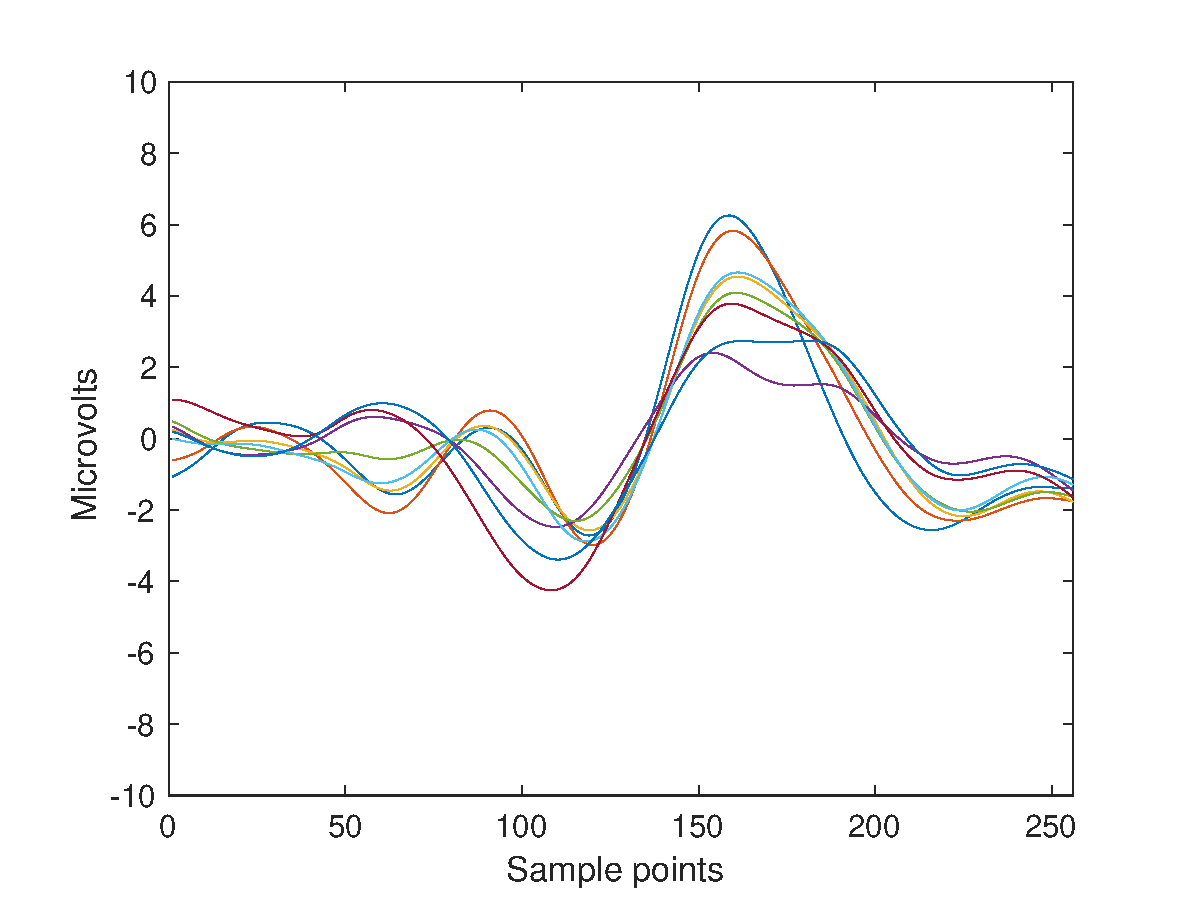
\includegraphics[width=6cm]{images/erptemplate1.eps}
\caption{ERP Template obtained from the point-to-point averaging of a P300 component of a subject obtained from the public dataset.}
\label{fig:erptemplate1}
\end{figure}

\subsubsection{Classification}

In order to classify we will use the same classifier for every method.  By doing this we will avoid 

\subsubsection{Parameters}

Each method has its own set of parameters which are optimized.  We will try to use an approach used in (matching pursuit paper for bci) where the best parameters are those which provide the best performance.

Hence, in order to obtain the right set of parameters for each method, an optimization problem was used fixing the injected signal to a gain of 3, and optimizing the parameters.

%%%%%%%%%%%%%%%%%%%%%%%%%%%%%%%%%%%%%%%%%%
\section{Results}
\label{section:results}

Results are shown in Table 1 and in Figure 1.  Table 1 shows the performance to identify each letter of the standard P300 Speller Matrix.   Figure 2 shows how the performance increase when averaging is implemented.


\begin{table}[H]
\caption{Accuracy levels obtained by a 3-fold cross validation. The values reported by the dataset publishers for Cz are reproduced here for comparison. Additionally, BCI accuracies for channel Cz can be seen as well as performance levels and their standard deviation obtained for the BPC, the best performing channel for each subject.}
\centering
%% \tablesize{} %% You can specify the fontsize here, e.g.  \tablesize{\footnotesize}. If commented out \small will be used.
\begin{tabular}{cc}
\toprule
\textbf{Method}	& \textbf{Single Trial Performance}	\\
\midrule
MP & 90 \\
PE & 89 \\
SHCC & 20 \\
\bottomrule
\end{tabular}
\label{tab:results}
\end{table}


\begin{figure}[H]
\centering
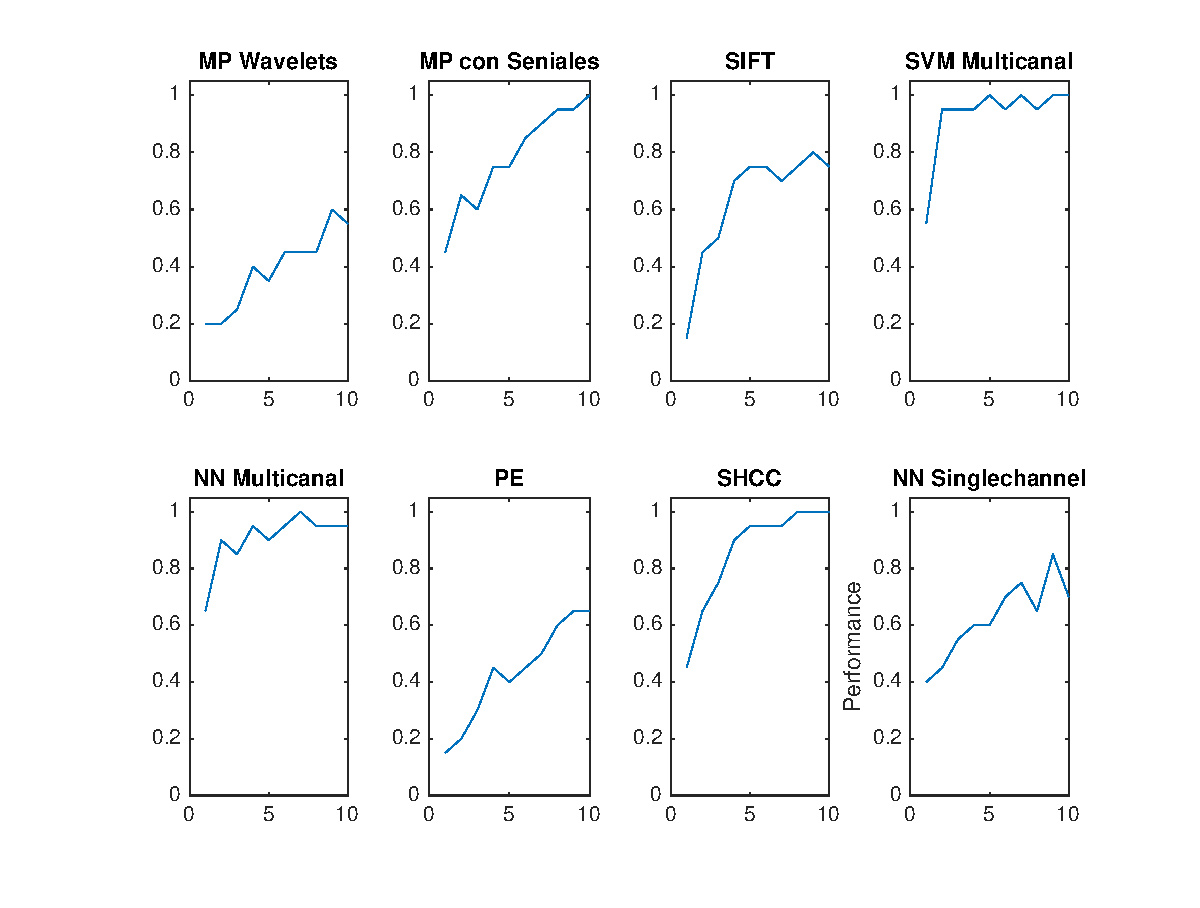
\includegraphics[width=6cm]{images/performance.eps}
\caption{Performance obtained from the different methods.}
\label{fig:performance}
\end{figure}


\begin{figure}[H]
\centering
\includegraphics[width=6cm]{images/P300Performance.eps}
\caption{Performance obtained from the different methods while averaging different trials.}
\label{fig:p300performance}
\end{figure}


%%%%%%%%%%%%%%%%%%%%%%%%%%%%%%%%%%%%%%%%%%
\section{Discussion}

In spite of all this, the conventional clinical method of observing the waveform is understood to be subjective and laborious because results depend on the technicians' experience and expertise.  The need for more objective measurements pushed the adoption of more automated means of decoding the signals and demanded a need for replication \citep{Thakor2004}.  This lead to the initial development of quantitative EEG, which however didn't replaced clinically the traditional approach which is still widespread.

This approach is relative common in chemical analysis (i.e. chemometrics Skoog, D.; West, D.; Holler, F. Analtyical Chemistry, An Introduction; Saunders: Philadelphia, 1994.), geology (sismic analysis), and quantitive financial analysis.  EKG, or Electrocardiogram, on the other hand, has been extensively processed and analyzed by waveform methods.
P,Q,R,S,T peaks in EKG analysis (REFERENCE) 

Dimensionality reduction which is truly applied when the waveform is actually formed.

We left out the segmetation issue which is itself a huge problem.  Where should I look from within the EEG trace ?

%%%%%%%%%%%%%%%%%%%%%%%%%%%%%%%%%%%%%%%%%%
\section{Conclusion}

The purpose of this work was twofold, (1) raise awareness about the utility of using automatic waveform-based methods to study EEG signals, (2) to provide an overview of the state-of-the-art of those methods, and (3) to verify and compare those methods.

Invasive methods remains an issue (referencia del paper de nature que muestra como causan deficits los implantes)


BCI as Assistive technology and BCI supplement natural motor output
The value of clinical focus, 
BCI reliability (WOkpaw and wolpaw).  Clinical EEG diagnosis may support a vast set of already understood knowledge which is based on identifying EEG patterns by their shape and that can lead to more robust implementation of BCI devices.

Let us now turn to the question posed in the title of this paper.

Successful approaches in Computer Vision or pattern recognition in other areas use a set of different features to compount ensemble classifiers.  All these methods had the advantage 
that they can truly map a visual component with a clinical meaning, assessed by a physician, and provide an automatic identification which can be constructed by the set of methods.  We believe this approach can be used to provide tools which are more meaningful to the clinical set.

Particularly considering BCI, this approach, in line with the general idea, can be used to foster BCI solutions that can help clinical settings.  Precisely for the same reasons.

More work has to be conducted in order to extend this methods to other patterns of waves.  

Berger H: tiber das Elektrenkephalogramm des Menschen, Archiv Psychiatr, 87 (1929) pp. 527-570.

%%%%%%%%%%%%%%%%%%%%%%%%%%%%%%%%%%%%%%%%%%
%\subsection{Subsection}
%
%\subsubsection{Subsubsection}
%
%Bulleted lists look like this:
%\begin{itemize}[leftmargin=*,labelsep=4mm]
%\item	First bullet
%\item	Second bullet
%\item	Third bullet
%\end{itemize}
%
%Numbered lists can be added as follows:
%\begin{enumerate}[leftmargin=*,labelsep=3mm]
%\item	First item
%\item	Second item
%\item	Third item
%\end{enumerate}
%
%The text continues here.



%%%%%%%%%%%%%%%%%%%%%%%%%%%%%%%%%%%%%%%%%%
\vspace{6pt} 

%%%%%%%%%%%%%%%%%%%%%%%%%%%%%%%%%%%%%%%%%%
%% optional
%\supplementary{The following are available online at www.mdpi.com/link, Figure S1: title, Table S1: title, Video S1: title.}

%%%%%%%%%%%%%%%%%%%%%%%%%%%%%%%%%%%%%%%%%%
\acknowledgments{This project was supported by the ITBACyT-15 funding program issued by ITBA University.}

%%%%%%%%%%%%%%%%%%%%%%%%%%%%%%%%%%%%%%%%%%
\authorcontributions{This projects is part of a the first author's PhD Thesis which is directed by Juan Miguel Santos and codirected by Ana Julia Villar.}

%%%%%%%%%%%%%%%%%%%%%%%%%%%%%%%%%%%%%%%%%%
%\conflictofinterests{The authors declare no conflict of interest.} 

%%%%%%%%%%%%%%%%%%%%%%%%%%%%%%%%%%%%%%%%%%
%% optional
\abbreviations{The following abbreviations are used in this manuscript:\\

\noindent EEG: electroencephalography\\
BCI: Brain Computer Interfaces\\
SNR: Signal to Noise Ratio\\
CNS: Central Nervous System\\
ALS: Amyotrophic Lateral Sclerosis\\
ERP: Event-Related Potential\\
P300: Positive deflection of an Event-Related Potential which occurs 300 ms after onset of stimulus\\
ITR: Information Transfer Rate\\
BTR: Bit Transfer Rate\\
SIFT: Scale Invariant Feature Transform\\
HOG: Histogram Of Gradients}

%%%%%%%%%%%%%%%%%%%%%%%%%%%%%%%%%%%%%%%%%%
%% optional
%\appendixtitles{no} %Leave argument "no" if all appendix headings stay EMPTY (then no dot is printed after "Appendix A"). If the appendix sections contain a heading then change the argument to "yes".
%\appendixsections{multiple} %Leave argument "multiple" if there are multiple sections. Then a counter is printed ("Appendix A?). If there is only one appendix section then change the argument to ?one? and no counter is printed (?Appendix?).
%\appendix
%\section{}
%The appendix is an optional section that can contain details and data supplemental to the main text. For example, explanations of experimental details that would disrupt the flow of the main text, but nonetheless remain crucial to understanding and reproducing the research shown; figures of replicates for experiments of which representative data is shown in the main text can be added here if brief, or as Supplementary data. Mathemtaical proofs of results not central to the paper can be added as an appendix.
%
%\section{}
%All appendix sections must be cited in the main text. In the appendixes, Figures, Tables, etc. should be labeled starting with `A', e.g., Figure A1, Figure A2, etc. 

%%%%%%%%%%%%%%%%%%%%%%%%%%%%%%%%%%%%%%%%%%
% Citations and References in Supplementary files are permitted provided that they also appear in the reference list here. 
\bibliographystyle{mdpi}

%=====================================
% References, variant A: internal bibliography
%=====================================
%\renewcommand\bibname{References}
%\begin{thebibliography}{999}
% Reference 1
%\bibitem{ref-journal}
%Lastname, F.; Author, T. The title of the cited article. {\em Journal Abbreviation} {\bf 2008}, {\em 10}, 142-149.
% Reference 2
%\bibitem{ref-book}
%Lastname, F.F.; Author, T. The title of the cited contribution. In {\em The Book Title}; Editor, F., Meditor, A., Eds.; Publishing House: City, Country, 2007; pp. 32-58.
%\end{thebibliography}

%=====================================
% References, variant B: external bibliography
%=====================================
\bibliography{sensors}

%%%%%%%%%%%%%%%%%%%%%%%%%%%%%%%%%%%%%%%%%%
%% optional
%\sampleavailability{Samples of the compounds ...... are available from the authors.}

%%%%%%%%%%%%%%%%%%%%%%%%%%%%%%%%%%%%%%%%%%
\end{document}